% exemples d'IR EAD et EAC
% exemples d'image de répertoire


\appendix
\part*{Annexes}
\addcontentsline{toc}{part}{Annexes}
\pagestyle{myheadings}
\markboth{Annexes}{Annexes}

Les annexes présentent à la fois les livrables réalisés durant le stage et des compléments à ce mémoire. Cette partie contient également les chemins de localisation des fichiers. Ils sont reproduits sur une \citecode{clé usb} et sur un dépôt \textit{Github} accessible à l'adresse suivante : \url{https://github.com/Lucaterre/L-TERRIEL_memoireDeStage_M2TNAH_ENC}.
\newpage
\thispagestyle{empty}
\chapter{Sources et Ecosystème Lectaurep}\label{source_lectaurep}

localisation : \citecode{/A-Sources\_et\_Ecosystème\_Lectaurep/} contenant :

\section{histoire du projet lectaurep}
localisation : \citecode{/A1-histoire\_projet\_lectaurep/} contenant :
\begin{itemize}
    \item \citecode{demande\_ocr\_Ollion.pdf} (pdf reproduit ci-dessous)
\end{itemize}


\section{Extraits du corpus des répertoires de notaires}
localisation : \citecode{A2-Extraits\_du\_corpus\_des\_répertoires\_de\_notaires/} contenant :
\begin{itemize}
    \item \citecode{exemple\_minute.jpg} ou Figure  \ref{fig:exemple_minute}
    \item \citecode{repertoire\_structure\_tableaux.png} ou Figure  \ref{fig:tableaux_repertoires}
\end{itemize}

\section{Outils généraux utilisés dans Lectaurep}

localisation : \citecode{A3-Outils\_de\_Lectaurep} contenant :
\begin{itemize}
    \item \citecode{Interface\_eScriptorium.png} ou Figure \ref{fig:appli_eScriptorium}
    \item \citecode{sharedocs.png} ou Figure \ref{fig:shareDocs}
    \item \citecode{blog\_lectaurep.png} ou Figure \ref{fig:blog_lectaurep}
\end{itemize}
% inclure les figures ici :

\newpage
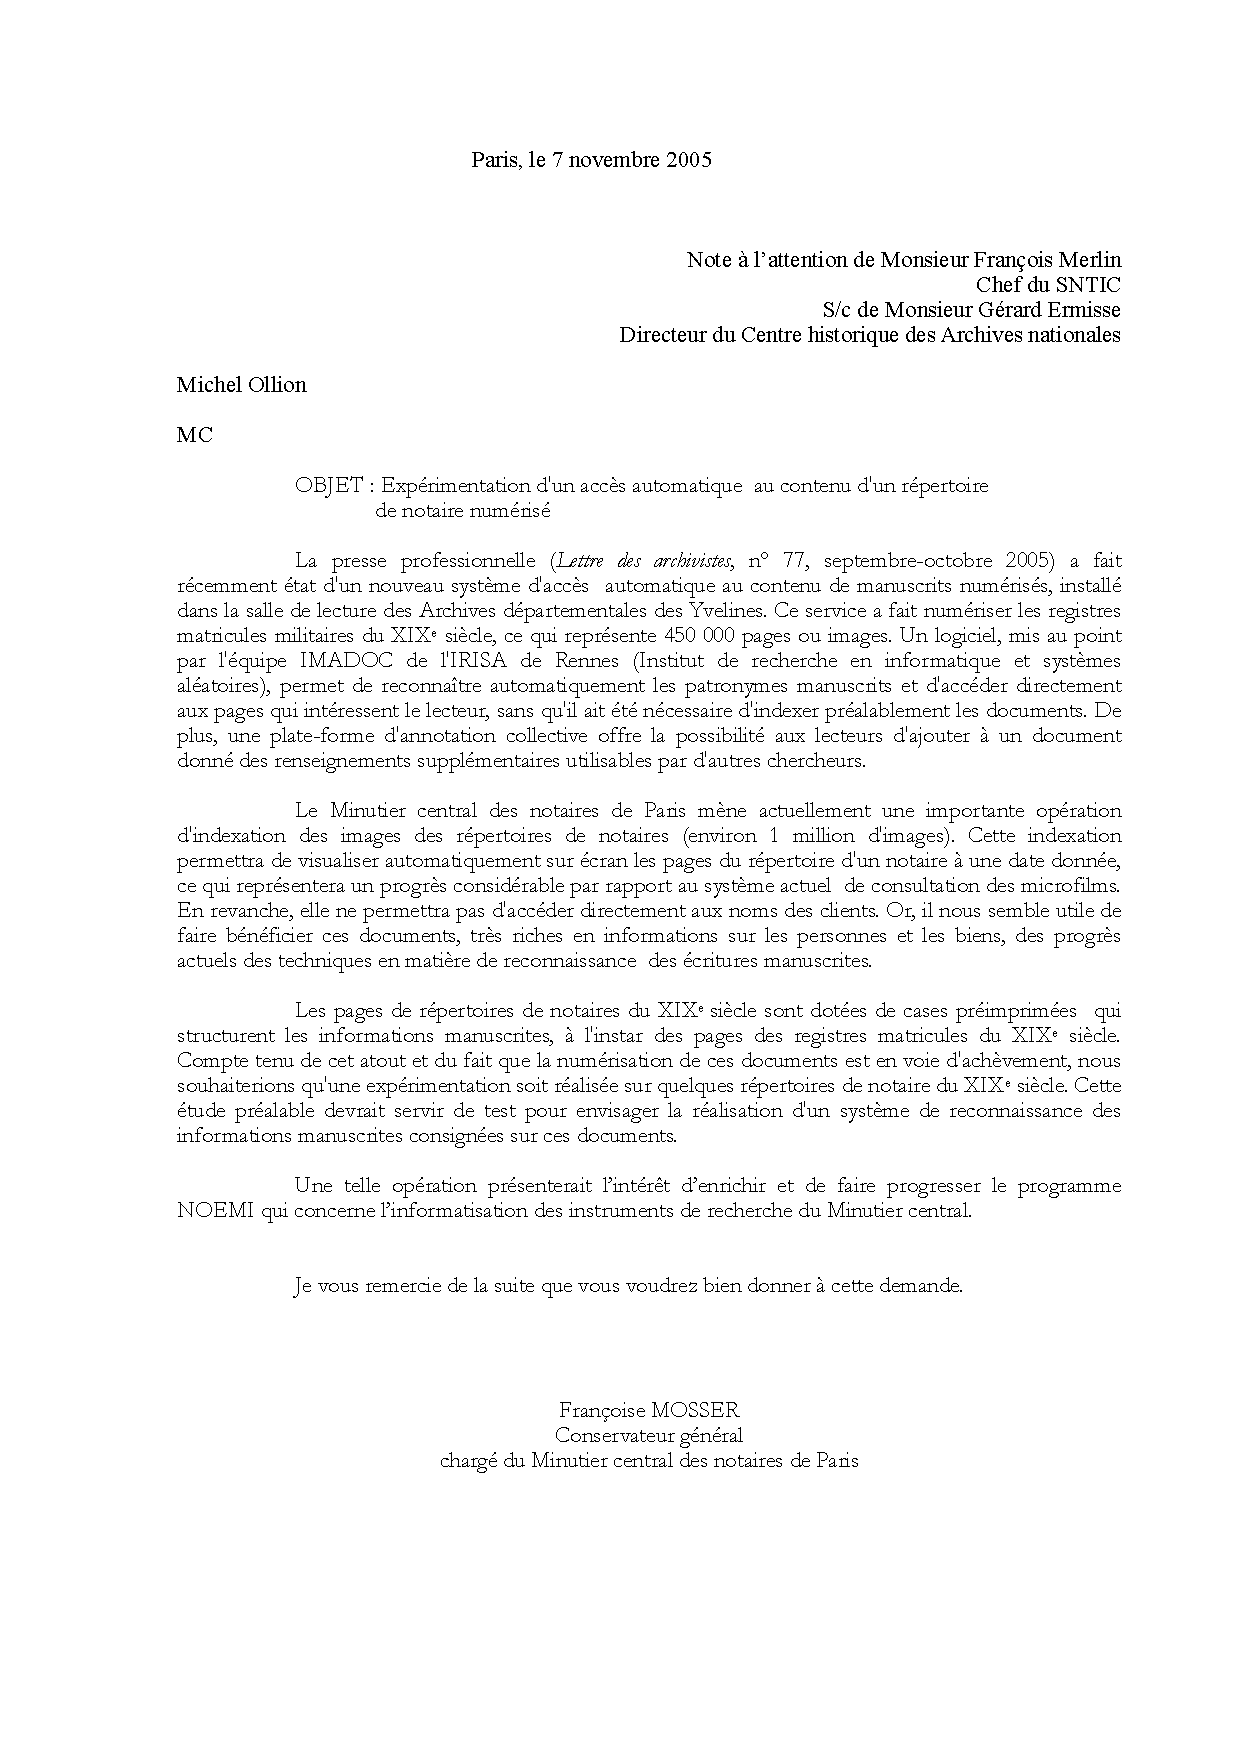
\includepdf{images_annexes/demande_ocr_Ollion.pdf}

\begin{figure}[h!]
    \centering
    \centerline{\fbox{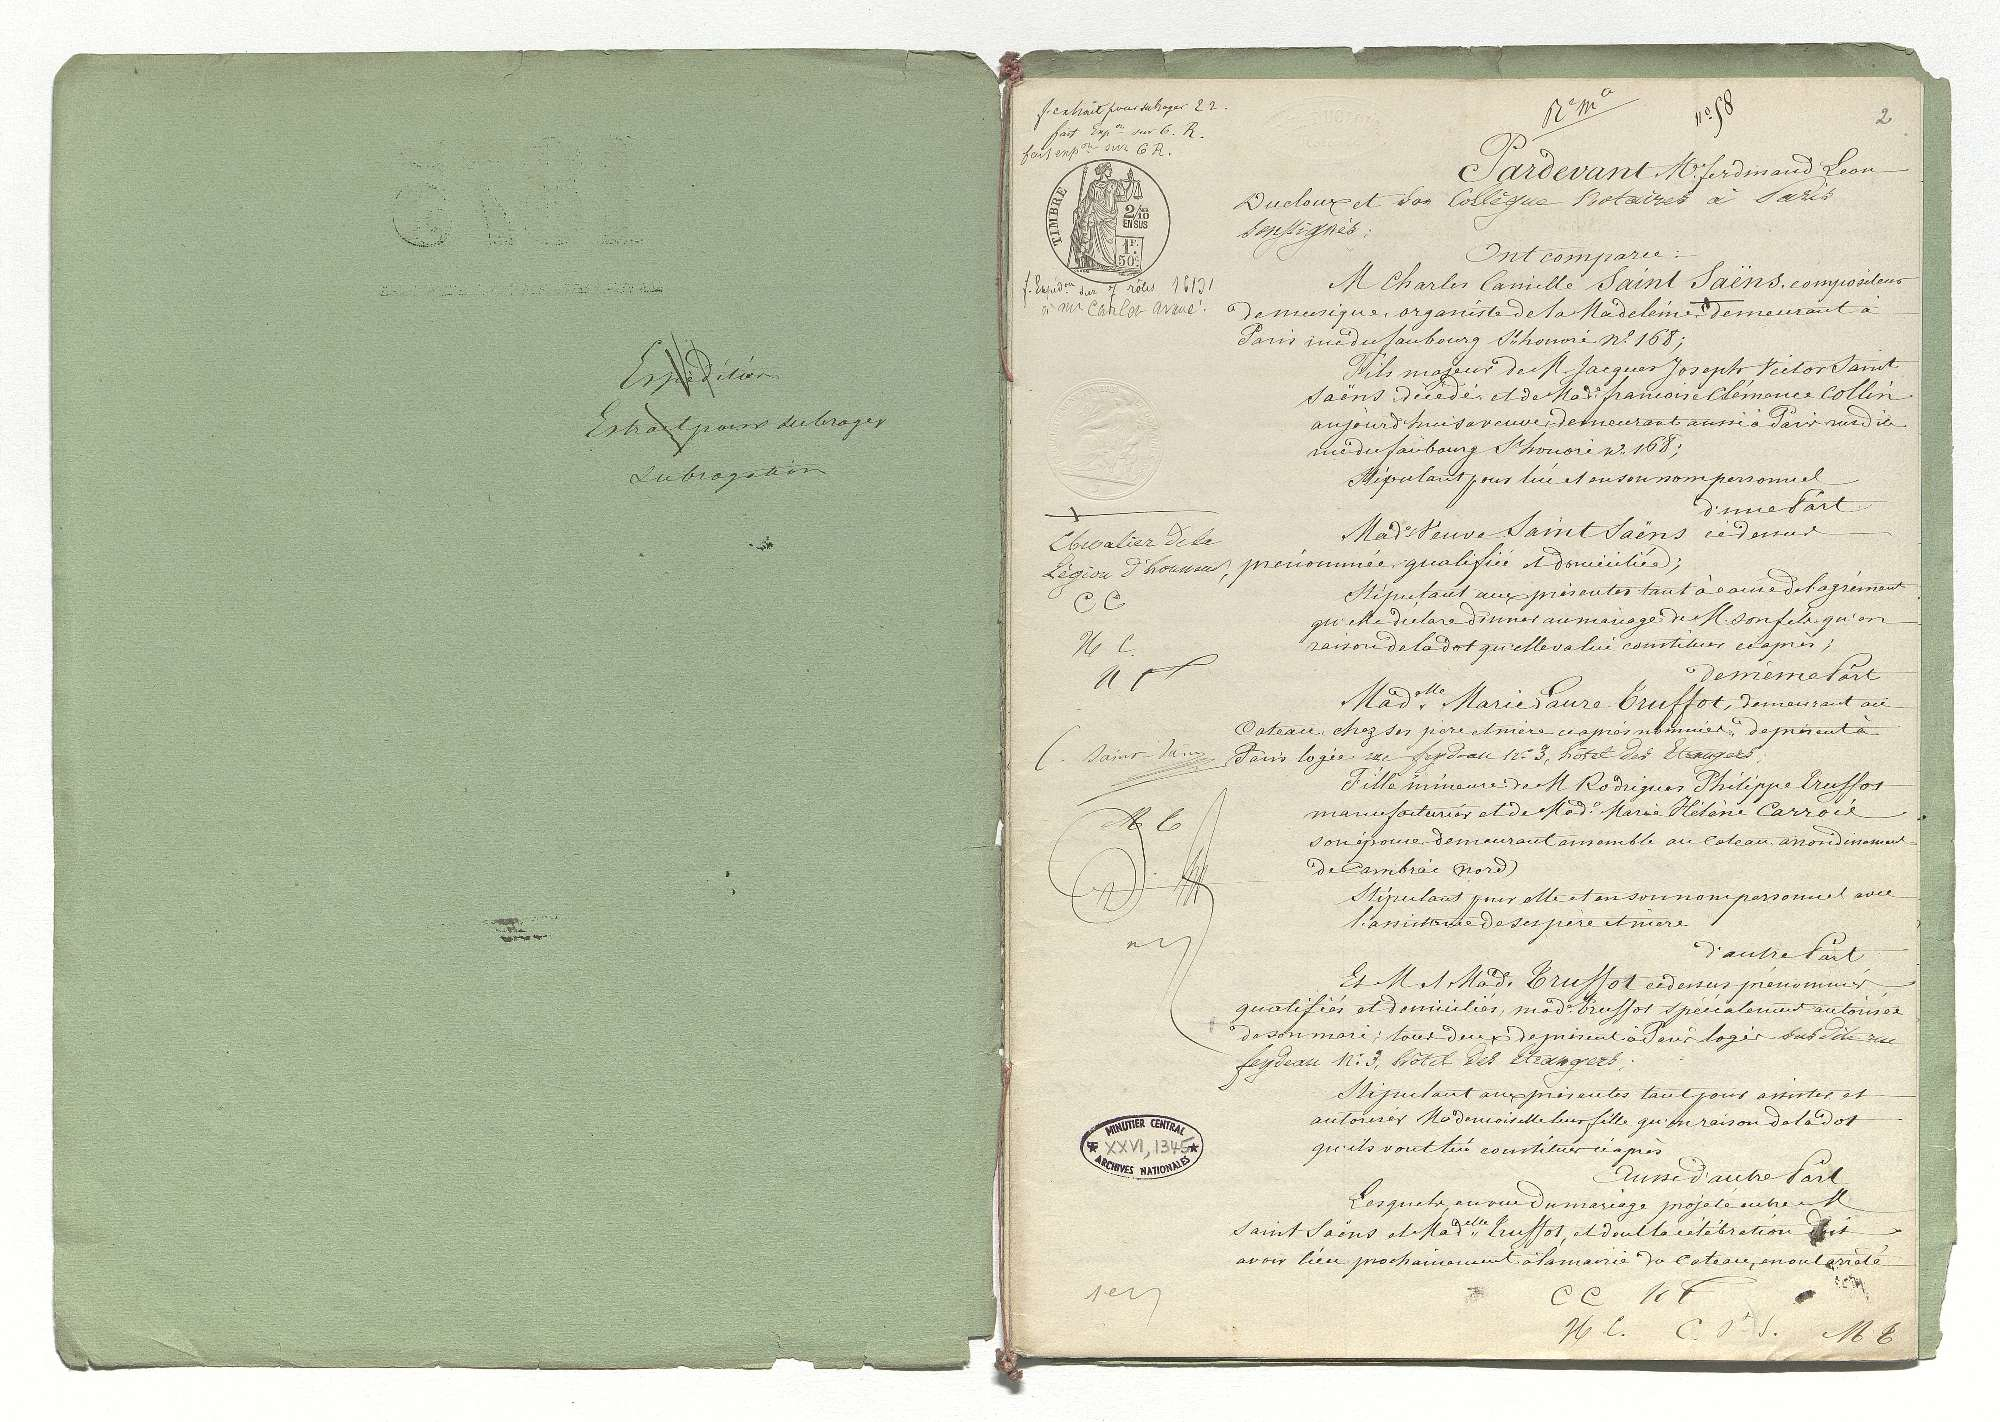
\includegraphics[width=19cm]{images_annexes/exemple_minute.jpg}}}
    \caption{Exemple de minute notariale \textcopyright Archives nationales/DMC, Minute \inquote{Contrat de mariage entre Charles Camille Saint-Saëns, compositeur de musique, organiste de la Madeleine demeurant au 168 rue du Faubourg Saint-Honoré, et Marie-Laure Truffot, fille de Rodrigue Truffot, manufacturier au Cateau-Cambrésis}, 18 janvier 1875,  MC/ET/XXVI/1345 (cote originale), MC/RS//872, lien vers la SIV : \url{https://www.siv.archives-nationales.culture.gouv.fr/siv/UD/FRAN_IR_041418/c1p6uqwjl1o3-xlv0cdl5wlgv}(consulté le 14/09/2020).}
    \label{fig:exemple_minute}
\end{figure}

\begin{figure}[h!]
    \centering
    \centerline{\fbox{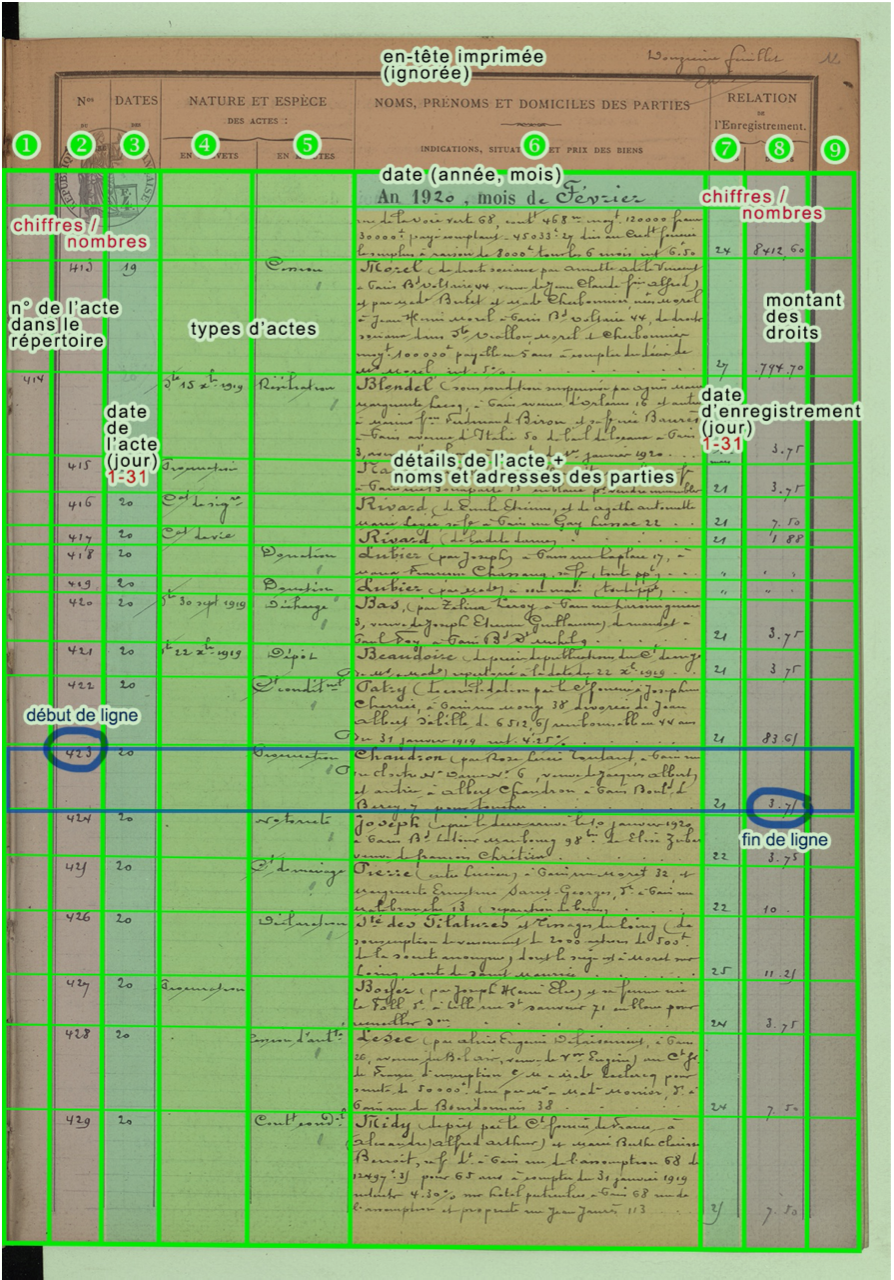
\includegraphics[width=14cm]{images_annexes/repertoire_structure_tableaux.png}}}
    \caption{Structuration en tableaux des répertoires \textcopyright \cite{bonhomme_defis_2018}, pp. 27.} 
    \label{fig:tableaux_repertoires}
\end{figure}

\begin{figure}[h]
    \centering
    \centerline{\fbox{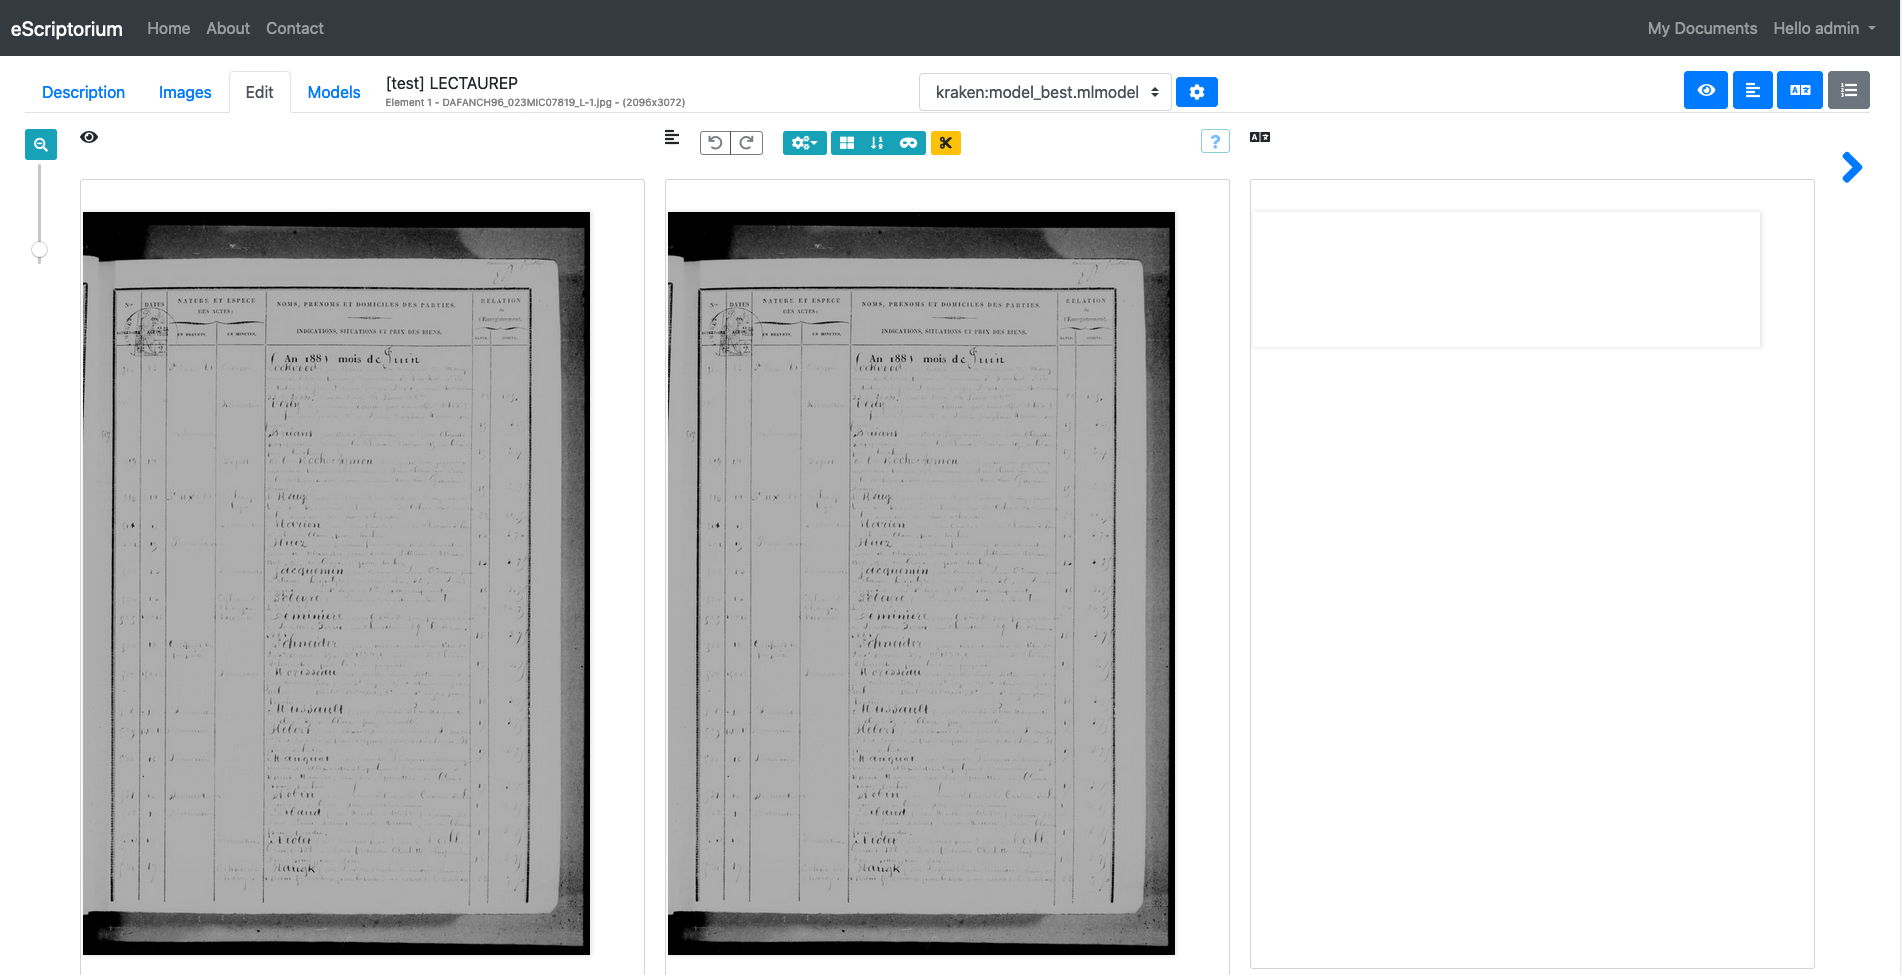
\includegraphics[width=18cm]{images_annexes/interface_eScriptorium.png}}}
    \caption{Application web eScriptorium \textcopyright L. Terriel, 2020, eScriptorium} 
    \label{fig:appli_eScriptorium}
\end{figure}

\begin{figure}[h]
    \centering
    \centerline{\fbox{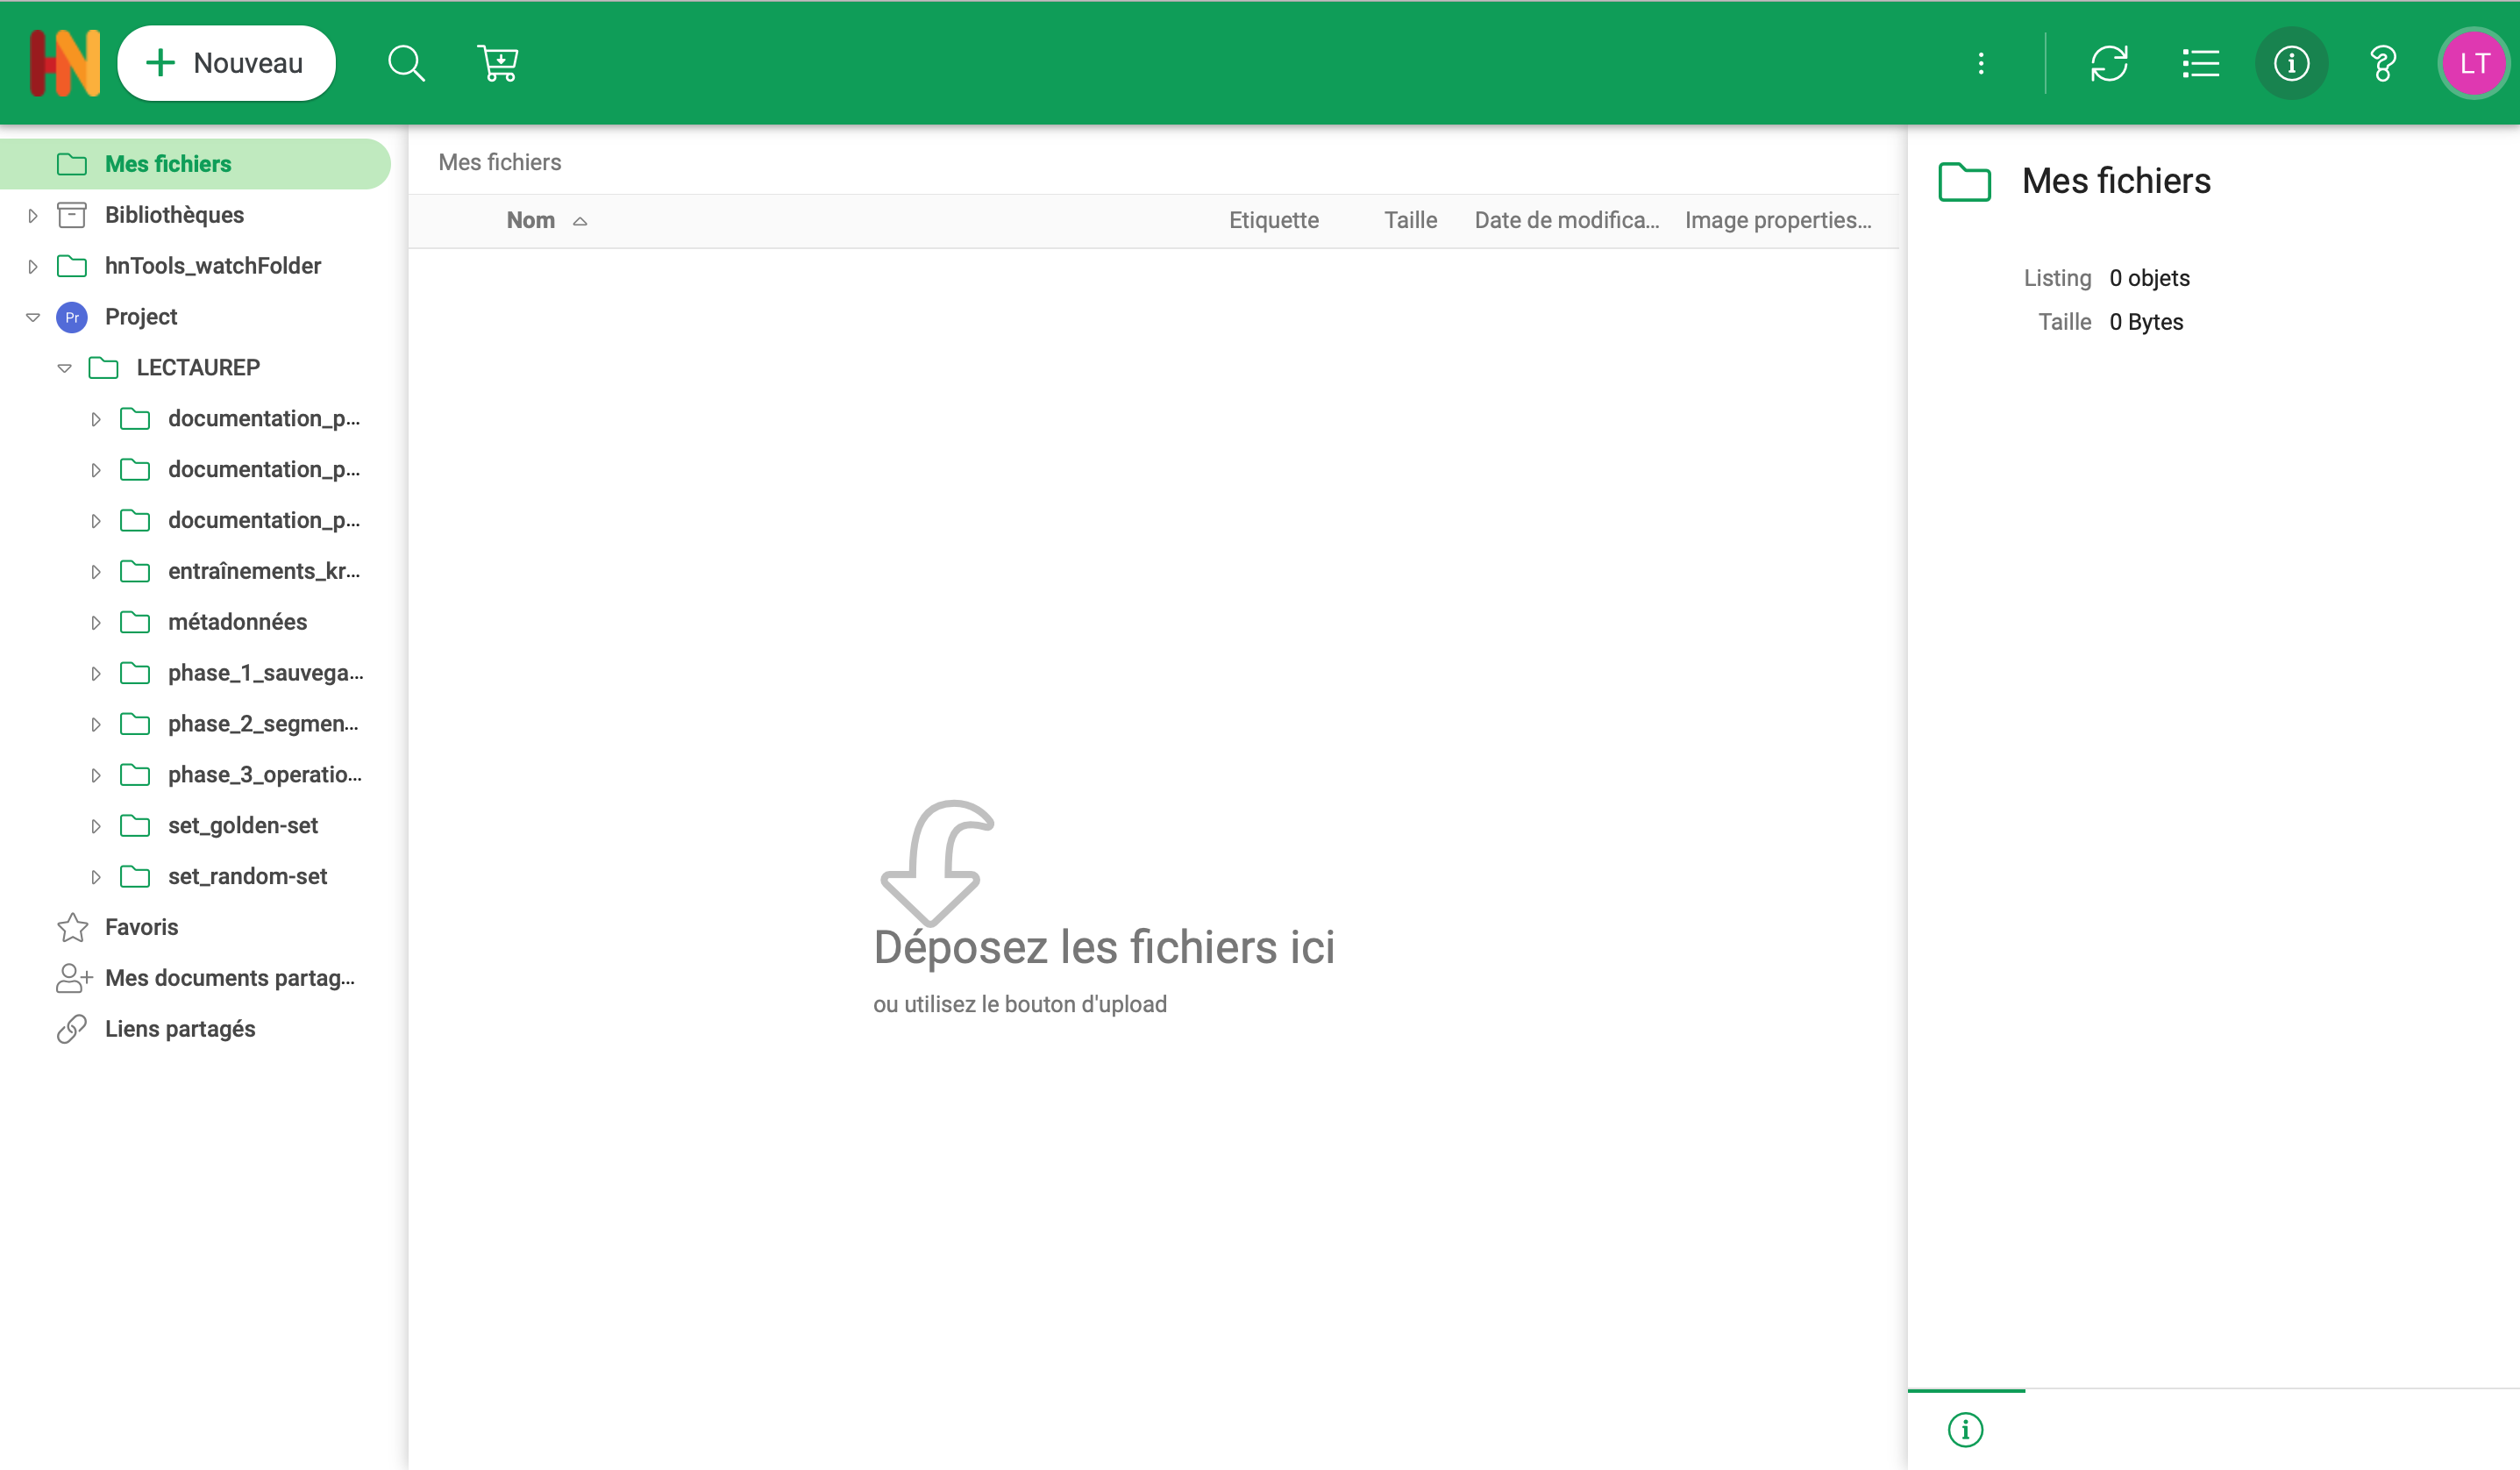
\includegraphics[width=18cm]{images_annexes/sharedocs.png}}}
    \caption{Exemple du \textit{Golden Set} et du \textit{Random Set} stockés sur l'espace \textit{Sharedocs} (Huma-num) \textcopyright L. Terriel, 2020, \textit{Sharedocs} (Huma-num)} 
    \label{fig:shareDocs}
\end{figure}

\begin{figure}[h!]
    \centering
    \centerline{\fbox{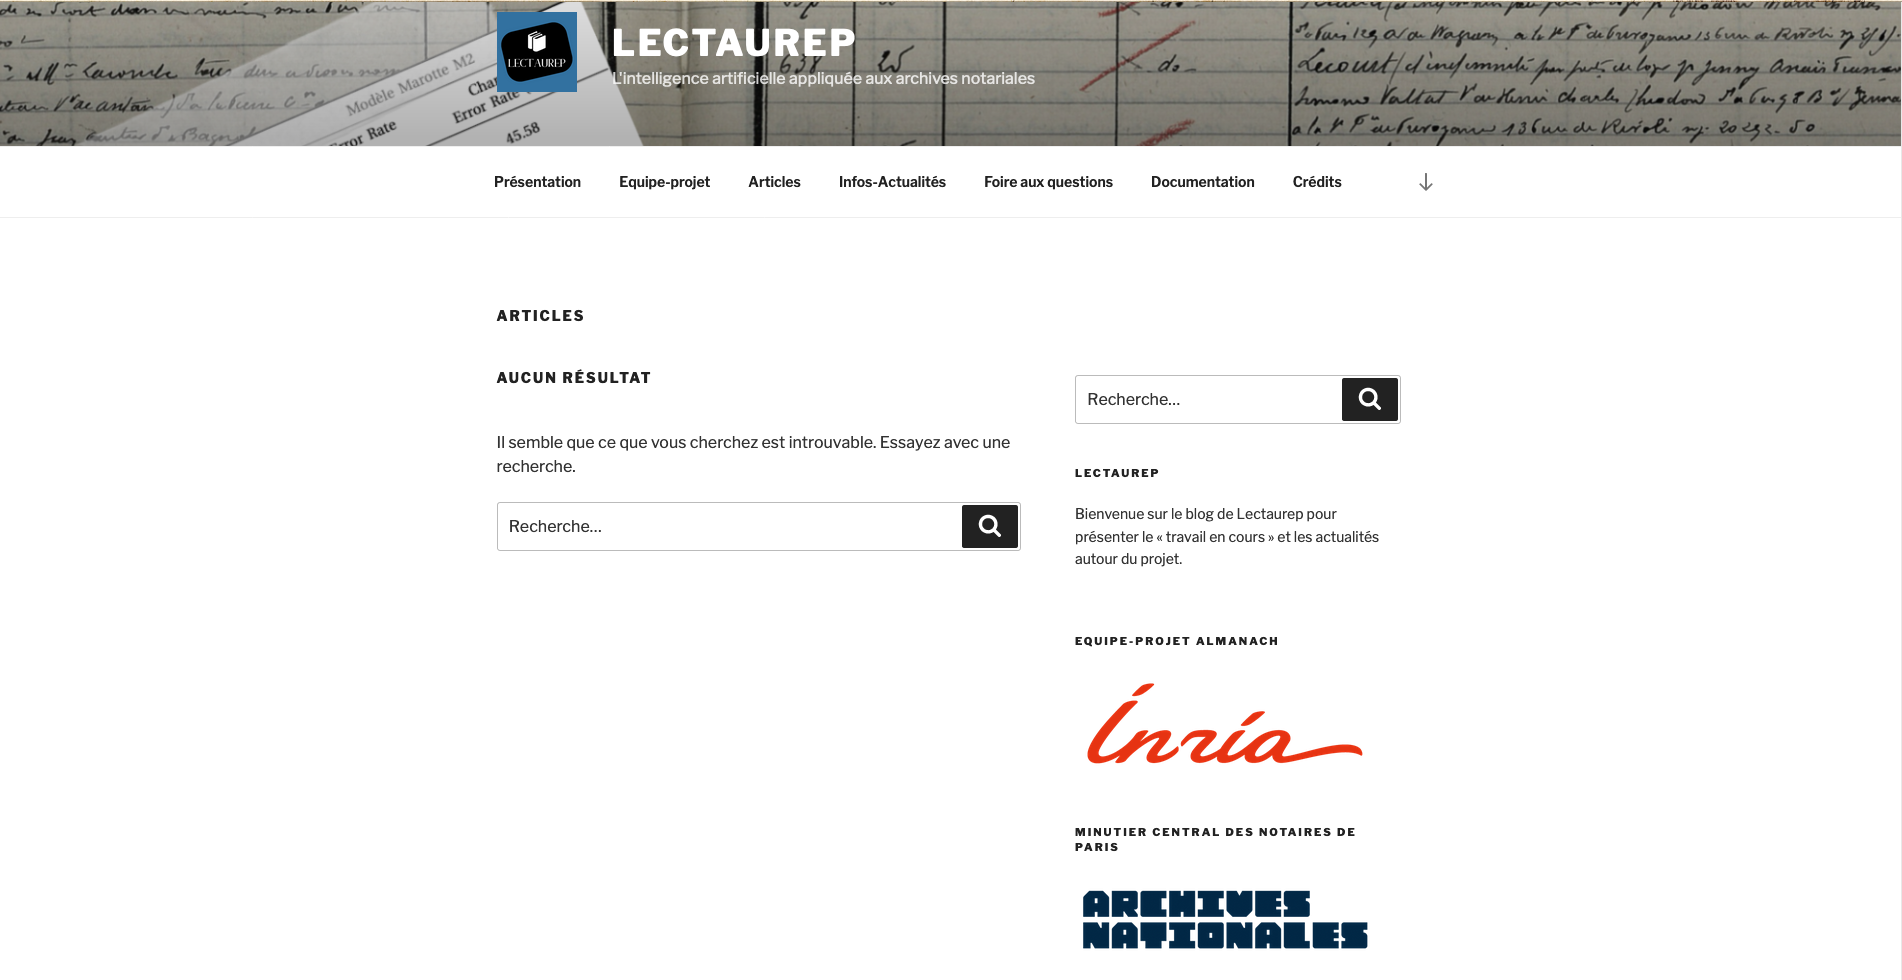
\includegraphics[width=18cm]{images_annexes/blog_lectaurep.png}}}
    \caption{Blog \textit{hypotheses.org} Lectaurep \textcopyright L. Terriel, blog \textit{hypotheses.org} Lectaurep}
    \label{fig:blog_lectaurep}
\end{figure}
\newpage
\thispagestyle{empty}
\chapter{Format pivot XML-TEI Lectaurep}\label{annexe_tei_pivot_prog}
localisation : \citecode{/B-Format\_pivot\_XML\_TEI\_Lectaurep} contenant :
\skip
\dirtree{%
.1 /B-Format\_pivot\_XML\_TEI\_Lectaurep/.
   .2 Doc/\DTcomment{Regroupe la documentation sur le projet du fichier pivot XML TEI pour Lectaurep}.
        .3 Modélisation\_et\_documentation\_format\_pivot/.
           .4 template\_pivot\_TEI\_lectaurep.xml\DTcomment{Canevas (\textit{template}) pour formaliser les attentes et les réflexions des acteurs pour l'inclusion des données et des métadonnées Lectaurep dans le fichier pivot XML-TEI.}.
           .4 Les ODD aux formats : XML, PDF et HTML.\DTcomment{La documentation standard TEI pour le fichier pivot XML-TEI Lectaurep.}.
           .4 oddbyexample.xsl\DTcomment{Une feuille de transformation XSL pour générer une nouvelle ODD à partir de la \textit{template} XML-TEI pivot.}.
        .3 Crosswalks\_vers\_TEI\DTcomment{Un ensemble de transformations XSL utiles vers les spécifications TEI et ALTO, issues de différents projets.}.
            .4 ALTO -> TEI.
            .4 EAD -> TEI (2 versions).
            .4 PAGE -> ALTO.
            .4 PAGE -> TEI.
   .2 Generator\_Lectaurep2TEI/\DTcomment{CLI Python permettant de simuler 
	                                     la conversion des données issues de Lectaurep (EAD-EAC, ALTO, EXIF) 
	                                     vers un fichier XML-TEI Pivot suivant les recommandations de l'ODD 
	                                     (voir le readme.md pour plus de détails).}.
        .3 Output/\DTcomment{Dossier dans lequel est généré la sortie du \textit{script}.}.
            .4  test\_legay\_tei.xml\DTcomment{Exemple de fichier pivot TEI Lectaurep de test généré en sortie du \textit{script}.}.
        .3 Sets\_test\_Legay/\DTcomment{Contient un ensemble de fichiers correspondant aux données fournies par Lectaurep pour tester le programme \textit{generator Lectaurep2TEI} et générer une première version du format pivot.}.
            .4  Data\_xml\_alto/\DTcomment{Fichiers XML ALTO correspondants aux transcriptions vérité terrain récupérées sur l'espace \textit{ShareDocs} relatives aux images numérisées du répertoire de notaire d'Ernest Legay (étude XXIII).}.
            .4  Data\_xml\_ead\_eac/\DTcomment{fichiers XML EAD et XML EAC-CPF correpondants aux instruments de recherche des répertoires du notaire Ernest Legay (étude XXIII) et notices producteurs récupérées sur la Salle des inventaires virtuels des Archives nationales.}.
                .5 FRAN\_IR\_041698.xml \DTcomment{IR \inquote{Minutes et répertoires du notaire Ernest LEGAY, 25 février 1875 - 14 mai 1902 (étude XXIII)}.}.
                .5 FRAN\_IR\_051379.xml \DTcomment{IR \inquote{Images des répertoires du notaire Ernest Legay pour l'étude XXIII}.}.
                .5 FRAN\_NP\_010150.xml \DTcomment{Notice producteur de l'étude XXIII.}.
                .5 FRAN\_NP\_011490.xml \DTcomment{Notice producteur de Legay, Ernest.}.
                .5 Schémas XML et DTD EAD et EAC-CPF.
            .4  images/\DTcomment{Images numérisées du répertoire de notaire d'Ernest Legay (étude XXIII) issues du \textit{Golden Set} de l'espace \textit{ShareDocs}.}.
        .3 generator\_utils/.\DTcomment{Ensemble des modules Python utiles au fonctionnement du CLI \textit{generator Lectaurep2TEI}. Pour les détails des fonctions consulter les \textit{docstrings} dans les \textit{scripts}.}.
            .4  \_\_init\_\_.py.
            .4  build\_utils.py.
            .4  extract\_utils.py.
            .4  validation\_utils.py.
        .3 pack\_schemaRNG/.\DTcomment{Doit accueillir à terme les schémas de validation Relax NG du fichier pivot XML-TEI Lectaurep.}.
            .4 tei\_all.rng.\DTcomment{Schéma Relax NG \textit{TEI ALL}.}.
        .3 Lectaurep\_ALTO2TEI.xsl.\DTcomment{Une feuille de transformation XSL ALTO vers TEI nécessaire pour le fonctionnement du \textit{script} principal. Pour plus de détails consulter la \textit{docstring} de la feuille.}.
        .3 Lectaurep\_EADEAC2TEI.xsl.\DTcomment{Une feuille de transformation XSL EAD/EAC vers TEI nécessaire pour le fonctionnement du \textit{script} principal. Pour les usages consulter la \textit{docstring}.}.
        .3 catalog\_alto.xml.\DTcomment{Fichier automatiquement créé par le \textit{script} principal, nécessaire pour l'usage de la fonction Xpath 2.0 \citecode{collection()} pour la feuille XSL \citecode{Lectaurep\_ALTO2TEI.xsl}}.
        .3 catalog\_ead\_eac.xml.Lectaurep\_ALTO2TEI.xsl\DTcomment{Fichier automatiquement créé par le \textit{script} principal, nécessaire pour l'usage de la fonction Xpath 2.0 \citecode{collection()} pour la feuille XSL \citecode{Lectaurep\_EADEAC2TEI.xsl}}.
        .3 generator\_Lectaurep2TEI\_logo.png.
        .3 inr\_logo\_grisbleu.png.
        .3 main.py.\DTcomment{\textit{Script} Python principal d'exécution du CLI \textit{generator Lectaurep2TEI}.}.
        .3 readme.md.\DTcomment{Documentation pour installer et lancer le programme.}.
        .3 requirements.txt.\DTcomment{Ensemble des \textit{packages} Python nécessaires à l'utilisation du CLI}.
        .3 snap\_generator.png.
        }
\newpage
\thispagestyle{empty}
\chapter{Application \textit{Kraken Benchmark}}\label{annexe_KB}
localisation : \citecode{/C-Application\_Kraken\_Benchmark} contenant :
\skip
\dirtree{%
.1 /C-Application\_Kraken\_Benchmark/.
   .2 Documentation-Reasearch/.\DTcomment{Contient les versions du \textit{notebook Jupyter} exposant les réflexions sur les métriques et les algorithmes utilisés dans l'application \textit{Kraken-Benchmark}.}.
    .3 Evaluation de la similarité entre deux séquences dans le contexte de la reconnaissance automatique de caractères.\DTcomment{\textit{Notebook} Jupyter en versions PDF, HTML et IPYNB (format natif).}. 
    .3 Ensemble d'images rattachées au \textit{notebook} Jupyter.
   .2 KB-app/.\DTcomment{Dossier contenant les fichiers pour faire fonctionner l'application \textit{\textit{Kraken-Benchmark}}.}.
    .3 STS\_Tools/.\DTcomment{Le \textit{package} Python \textit{Sequences to Similarity} créé pour l'application \textit{\textit{Kraken-Benchmark}} contient deux modules Python.}.
        .4 STSig.py.\DTcomment{Module Python \textit{Sequences To Signals} (en cours de développement); module pour créer des visualisations et des métriques expérimentales pour comparer deux chaînes de caractères.}.
        .4 SynSemTS.py.\DTcomment{Module Python \textit{Syntactic Semantic To Similarity} qui contient la plupart des métriques (syntaxiques et sémantiques) et les visualisations associées; utilisé dans l'application pour l'analyse de deux chaînes de caractères correspondant à la vérité terrain et la transcription issue du système HTR.}.
        .4  \_\_init\_\_.py.
    .3 kb\_report/.\DTcomment{Dossier contenant les fichiers pour la gestion de la partie affichage dans le navigateur de l'application via le \textit{package} \textit{Flask}.}.
        .4  static/.\DTcomment{Contient les images de l'application à afficher dans le navigateur.}.
        .4  templates/.\DTcomment{Contient les pages HTML de l'application.}.
        .4  \_\_init\_\_.py.
        .4  routing.py\DTcomment{\textit{Script} Python qui contient les différentes routes URL de l'application.}.
    .3 kb\_utils/.\DTcomment{Dossier contenant un module Python nécessaire au fonctionnement de l'application.}.
        .4  \_\_init\_\_.py.
        .4  kb\_utils.py.\DTcomment{Module Python contenant des fonctions utiles au fonctionnement de l'application.}.
    .3 environment.yml.\DTcomment{Fichier pour la création d'un environnement virtuel \textit{Conda} contenant les \textit{packages} Python nécessaires.}.
    .3 kraken\_benchmark.py.\DTcomment{\textit{Script} principal pour l'exécution de l'application \textit{Kraken-Benchmark}.}.
   .2 sets\_test/.\DTcomment{Jeux de fichiers pour effectuer des tests dans \textit{Kraken-Benchmark} et \textit{scripts} Python complémentaires.}.
    .3 jules\_verne\_set\_test/.\DTcomment{Jeux de données utilisés pour les tests fonctionnels de l'application.}.
        .4  images/.\DTcomment{Contient des numérisations (formats \citecode{.jpeg}) de l'ouvrage \textit{Voyage au centre de la terre} récupérés sur \og Gallica\fg{}}.
        .4  dataset\_GT/.\DTcomment{Contient les vérités terrains en format texte brut utilisées pour comparer les résultats issus de l'HTR de \textit{Kraken-Benchmark}. Édités à partir du CLI Kraken.}.
        .4  model/.\DTcomment{Contient le modèle (format \citecode{.mlmodel}) entraîné sur le CLI Kraken pour réaliser l'OCR dans \textit{Kraken-Benchmark} sur le \textit{set} de numérisations de \textit{Voyage au centre de la terre}.}.
    .3 sets\_tests\_lectaurep/.\DTcomment{Jeux de données utilisés pour tester les modèles de transcription issus du CLI Kraken sur des images de répertoires de notaires sélectionnées pour leurs particularismes (pour plus de détails sur les sets d'images et les modèles HTR utilisés voir le fichier \citecode{CR\_tests\_lectaurep\_KB.md}) pour évaluer la qualité des transcriptions. pour plus de précisions, Cf. section \ref{tests_KB_lectaurep}}.
        .4  different\_control\_set/.\DTcomment{Contient les transcriptions vérité terrains (\citecode{GT} et les images).}.
        .4  homogeneous\_control\_set/.\DTcomment{Contient les transcriptions vérité terrains (\citecode{GT} et les images).}.
        .4  set\_material\_defects/.\DTcomment{Contient les transcriptions vérité terrains (\citecode{GT} et les images).}.
        .4  set\_writing\_defects/.\DTcomment{Contient les transcriptions vérité terrains (\citecode{GT} et les images).}.
        .4  snaps\_tests\_lectaurep/.\DTcomment{Contient des sauvegardes des pages HTML de l'application \textit{Kraken-Benchmark} réalisées lors des différents tests Lectaurep.}.
            .5 report\_html/.\DTcomment{Contient des captures de la page d'accueil de \textit{Kraken-Benchmark} avec les principales métriques.}.
            .5 versus\_text\_html/.\DTcomment{Contient des captures de la fonctionnalité \textit{versus text} (comparaison de la vérité terrain et de la transcription HTR dans \textit{Kraken-Benchmark}).}.
        .4  models/.\DTcomment{Contient les modèles HTR, entraînés avec le CLI \textit{Kraken}, et utilisés sur les différents jeux de données.}.
        .4  CR\_tests\_lectaurep\_KB.md\DTcomment{Compte-rendu présentant le déroulement des tests, la description des sets de tests, des modèles et des résultats des expériences.}.
        .4  details\_data\_average\_tests\_model\_test\_lectaurep\_bin\_accuracy\_6064.mlmodel - Feuille 1.pdf\DTcomment{Fichier PDF présentant la moyenne des résultats des tests avec le modèle 6064, utilisé pour le graphique radar.}.
        .4   details\_data\_average\_tests\_model\_test\_lectaurep\_bin\_accuracy\_8164.mlmodel - Feuille 1.pdf\DTcomment{Fichier PDF présentant la moyenne des résultats des tests avec le modèle 8164, utilisé pour le graphique radar.}.
        .4  radar\_test\_II\_model\_0-8164.png\DTcomment{Graphique du model 8164.}.
        .4  radar\_test\_I\_model\_0-6064.png\DTcomment{Graphique du model 6064.}.
    .3 alto2text.py.\DTcomment{\textit{Script} Python adapté, provenant de la \textit{StaatsbibliothekBerlin} permettant la conversion de certaines transcriptions vérités terrains en XML ALTO vers des fichiers texte brut.}.
    .3 radar\_graph.py.\DTcomment{\textit{Script} Python adapté permettant la génération d'un graphique radar, utile pour le rapport concernant les tests spécifiques à Lectaurep durant le stage.}.
   .2 README.md.\DTcomment{Présentation et documentation principale de l'application pour l'installation et l'utilisation de \textit{Kraken-Benshmark}.}.
   .2 ci-test.sh.\DTcomment{\textit{Script} Bash (Alix Chagué) pour configurer les tests de l'application (avec le logiciel \citecode{Pylint}) doit accueillir l'appel des tests unitaires.}.
   .2 .pylintrc.\DTcomment{Fichier pour configurer \citecode{Pylint}.}.
   .2 requirements.txt.\DTcomment{Fichier d'installation des \textit{packages}, utilisé exclusivement par le \textit{script} \citecode{ci-test.sh}.}.
   }
\newpage
\thispagestyle{empty}
\chapter{Documents de travail pour le fichier pivot XML-TEI Lectaurep}\label{doc_ax_tei_pivot}
localisation : \citecode{/D-Doc\_travail\_pivot\_tei\_lectaurep} contenant :

\begin{itemize}
    \item \citecode{modèle\_metadonnées\_vise\_V4.png} ou Figure \ref{fig:modele_vise_V4}
    \item \citecode{Generateur-XML-TEI.png} ou Figure \ref{fig:generateur_tei}
\end{itemize}

% Figures en dessous : 

\begin{figure}
  \begin{sideways}
    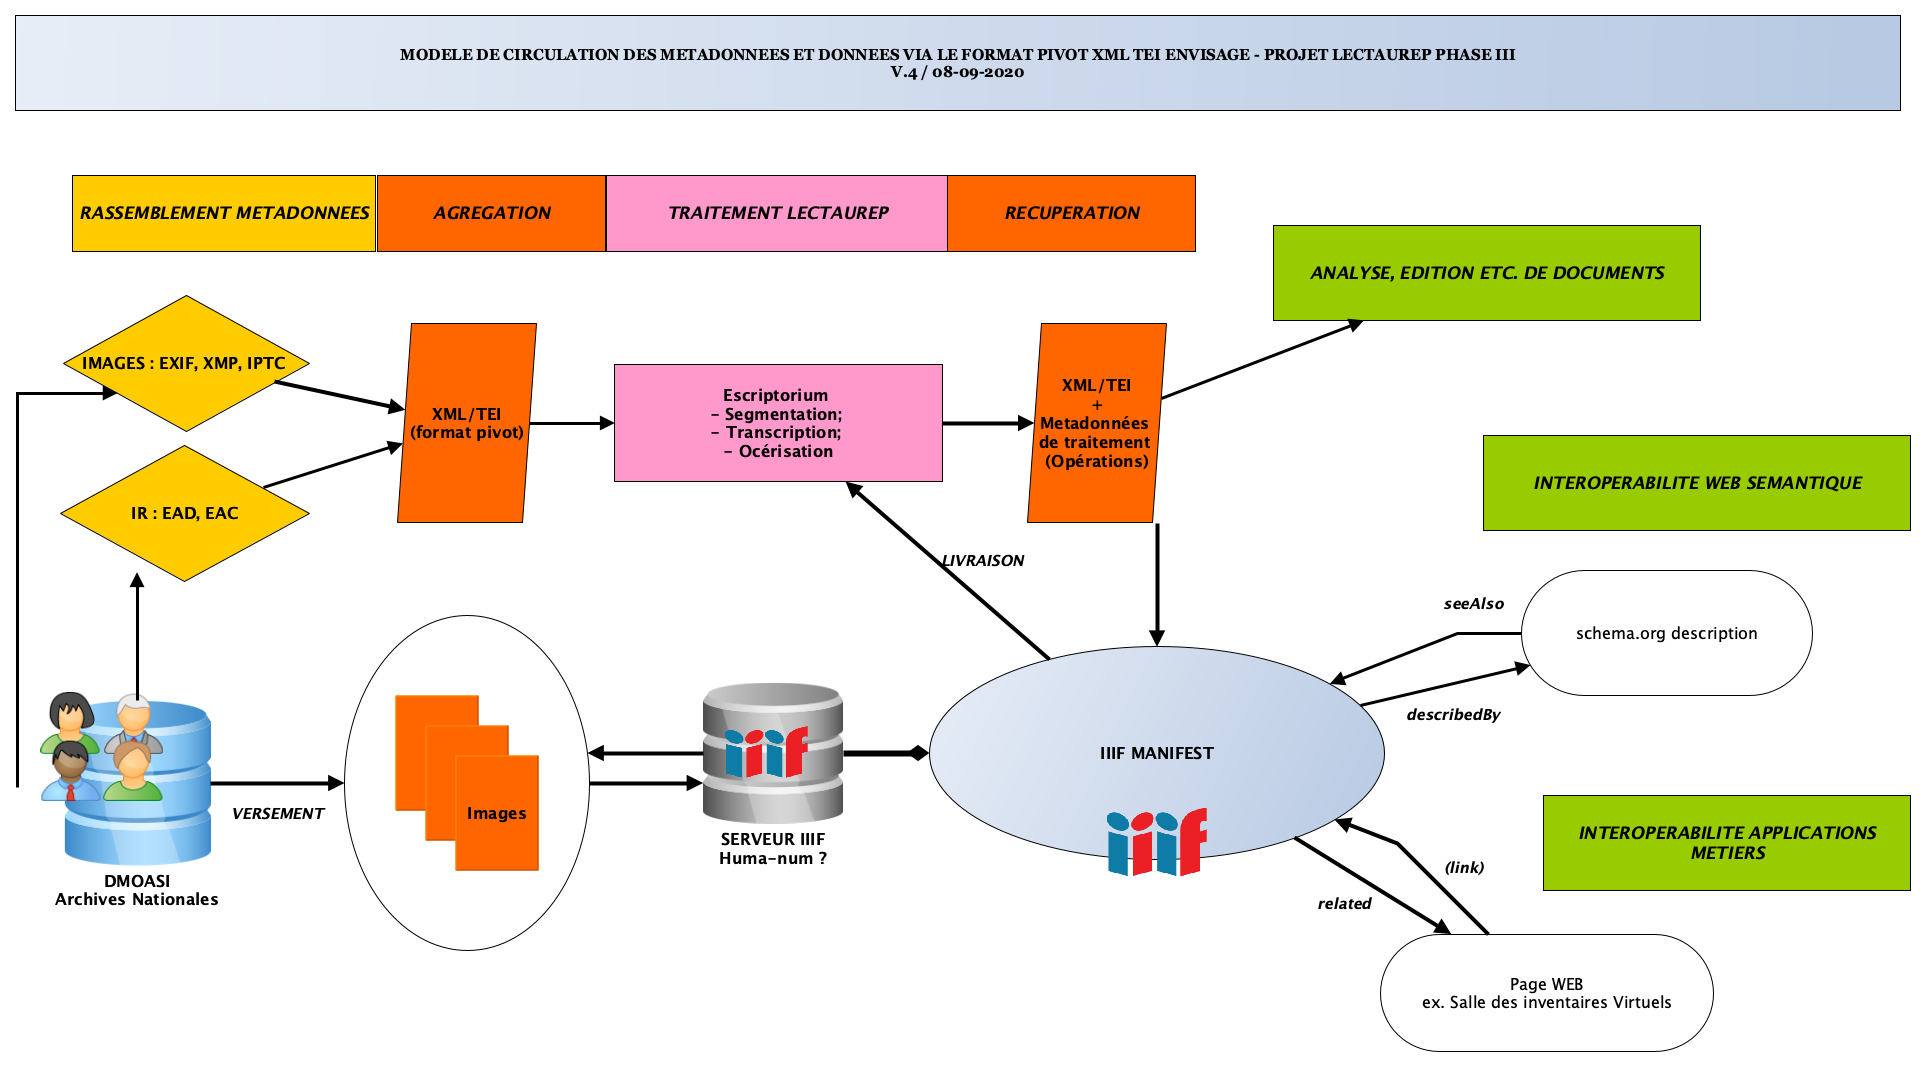
\includegraphics[width=24cm, height=16cm]{images_annexes/modèle_metadonnées_vise_V4.png}
  \end{sideways}
  \centering
  \caption{Schématisation du modèle de circulation des données dans \textit{eScriptorium} souhaité par Lectaurep à terme  \textcopyright L. Terriel, 2020, yEd}
  \label{fig:modele_vise_V4}
\end{figure}

\begin{figure}
    \centering
    \centerline{\fbox{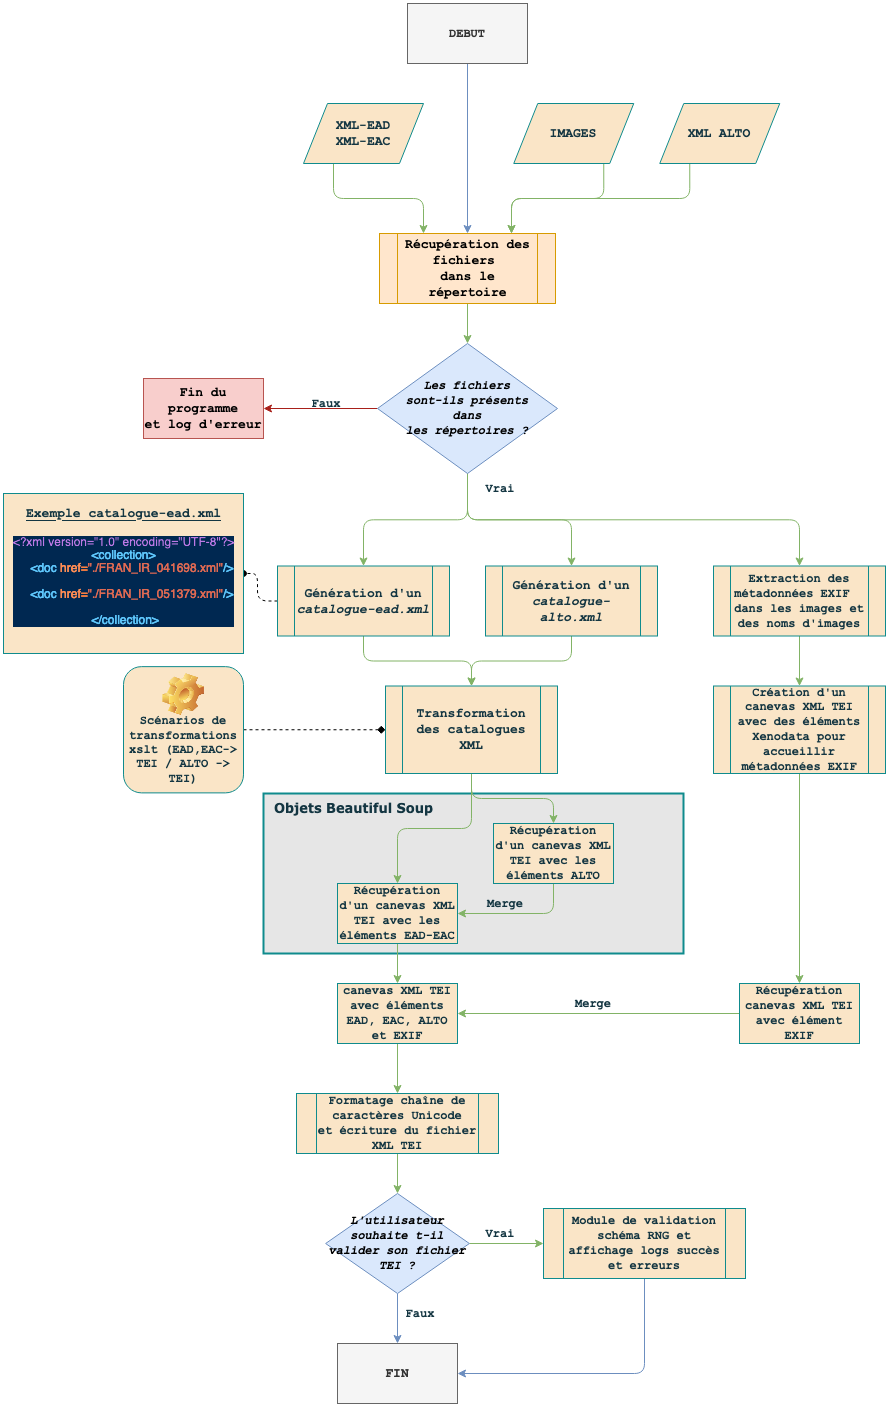
\includegraphics[width=18cm, height=22.5cm]{images_annexes/Generateur-XML-TEI.png}}}
    \caption{Algorigramme du programme \textit{Generator Lectaurep-TEI} pour simuler la visualisation d'un fichier XML-TEI pivot comprenant des données provenant de fichiers XML ALTO, EAD et EAC-CPF et des métadonnées EXIF provenant d'images.   \textcopyright L. Terriel, 2020, Diagrams.net}
    \label{fig:generateur_tei}
\end{figure}

\chapter{Documents de travail pour \textit{\textit{Kraken-Benchmark}}}\label{doc_ax_kb}
localisation : \citecode{/E-Doc\_travail\_KB} contenant :

\begin{itemize}
    \item \citecode{detail-model-transkribus.png} ou Figure \ref{fig:details-model-transkribus}
    \item \citecode{compare-texts-transkribus.png} ou Figure \ref{fig:compare-texts-transkribus}
    \item \citecode{Kraken-Benchmark\_modelisation.png} ou Figure \ref{fig:algo-kb}
\end{itemize}

% Figures en dessous :
\begin{figure}
    \centering
    \centerline{\fbox{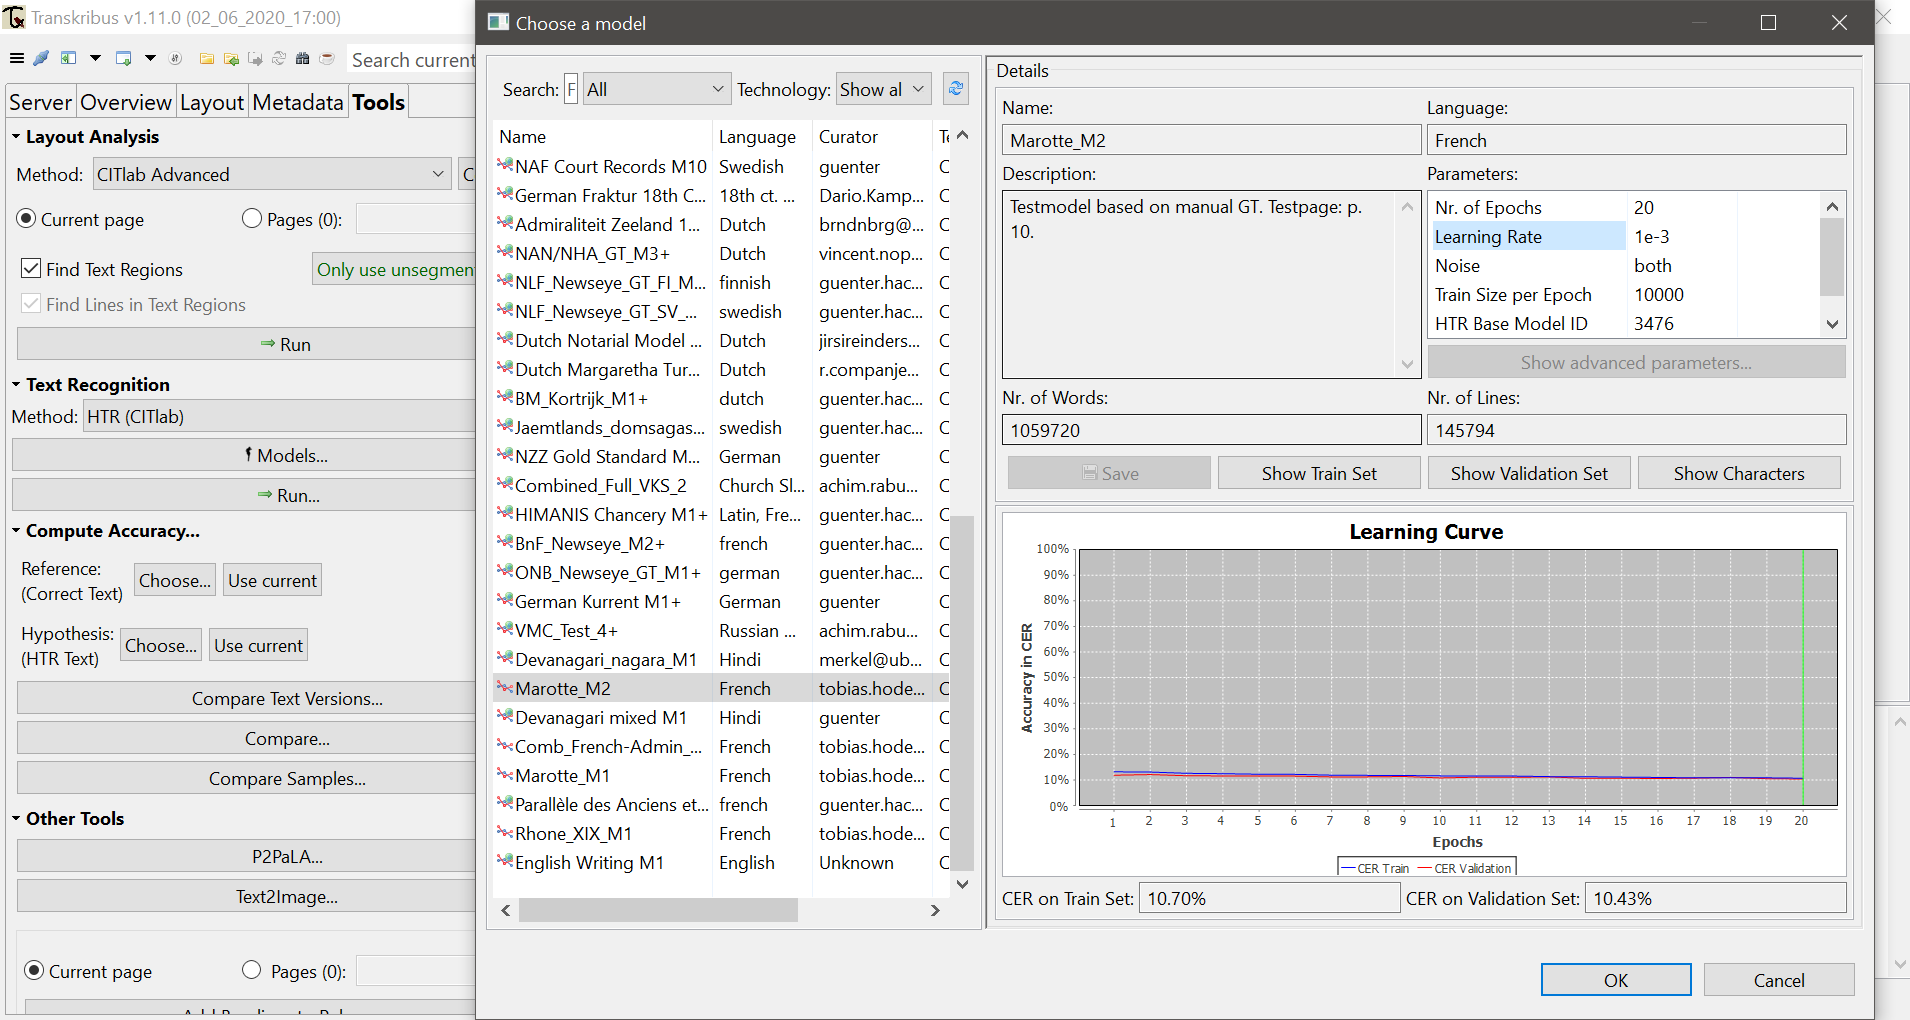
\includegraphics[width=18cm]{images_annexes/detail-model-transkribus.png}}}
    \caption{Fenêtre pour visualiser des détails concernant le modèle envoyé dans l'interface \textit{Transkribus} \textcopyright A. Chague, 2020, \textit{Transkribus}}
    \label{fig:details-model-transkribus}
\end{figure}

\begin{figure}
    \centering
    \centerline{\fbox{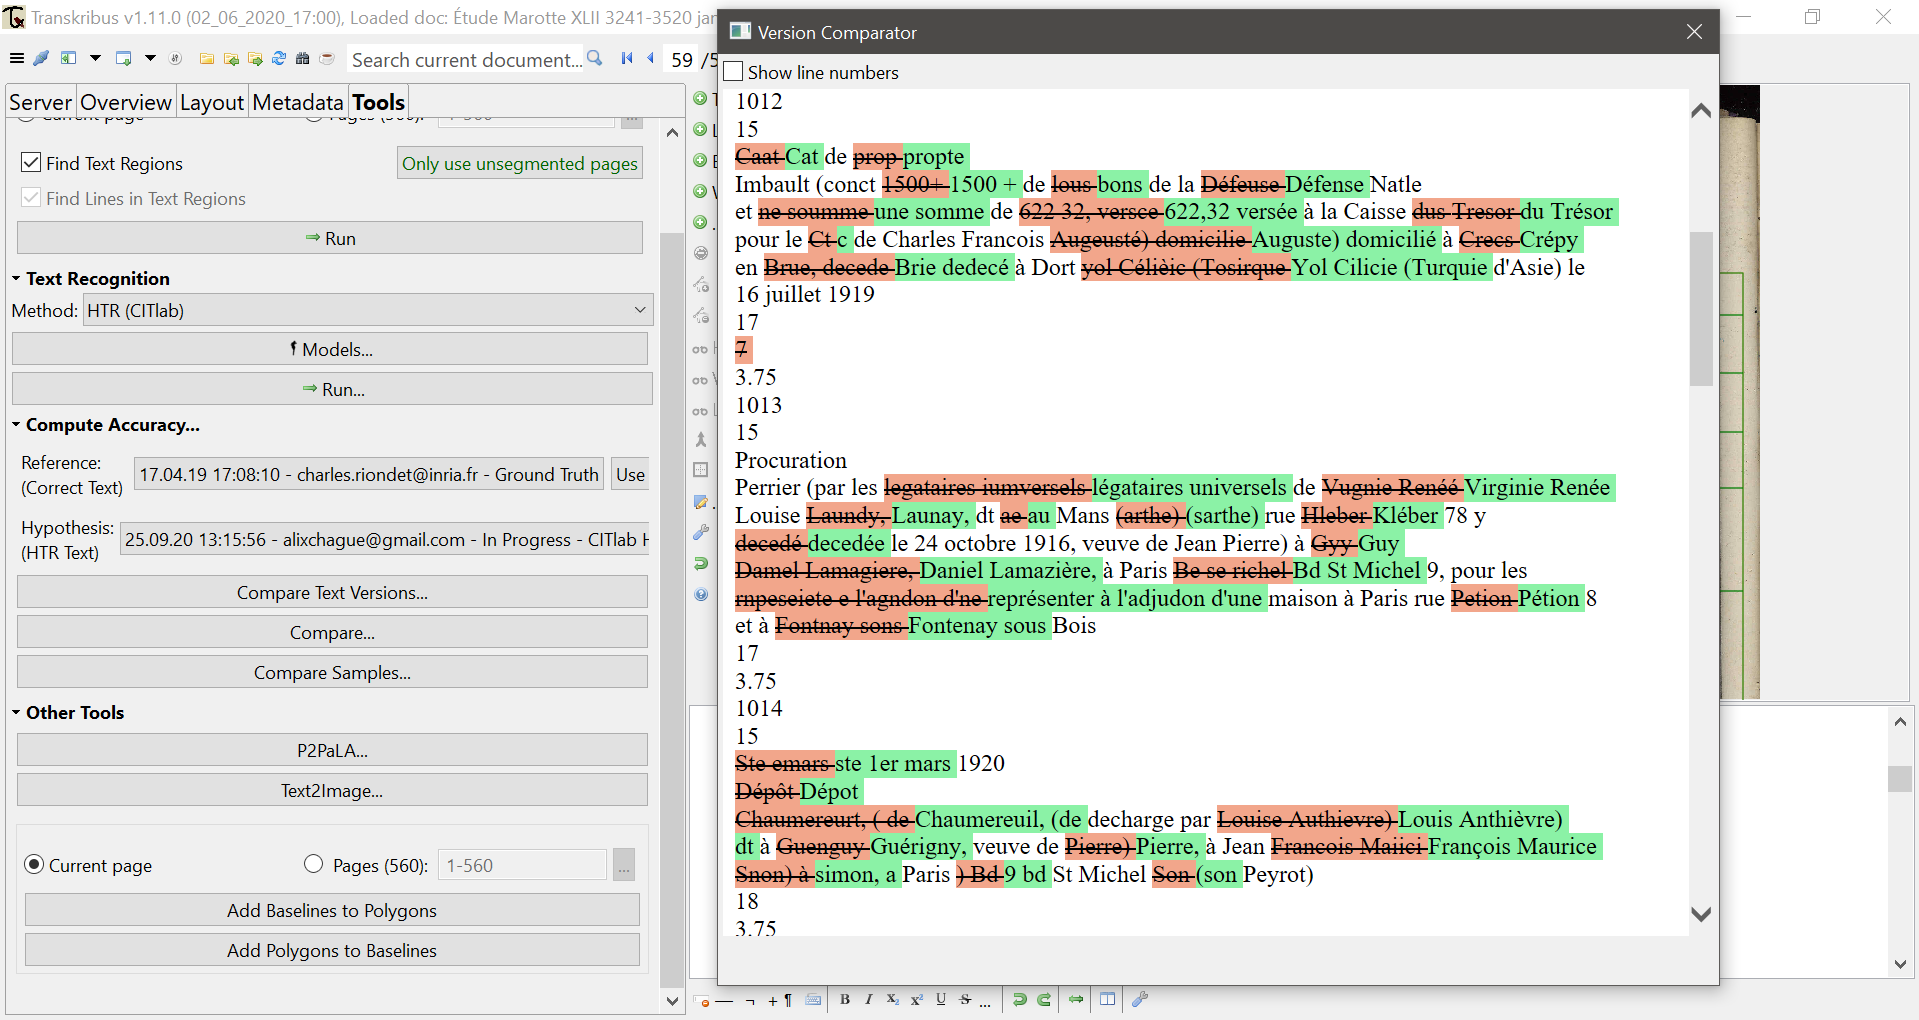
\includegraphics[width=18cm]{images_annexes/compare-texts-transkribus.png}}}
    \caption{Fenêtre pour comparer la référence et la prédiction dans l'interface \textit{Transkribus} \textcopyright A. Chague, 2020, \textit{Transkribus}}
    \label{fig:compare-texts-transkribus}
\end{figure}

\begin{figure}
    \centering
    \centerline{\fbox{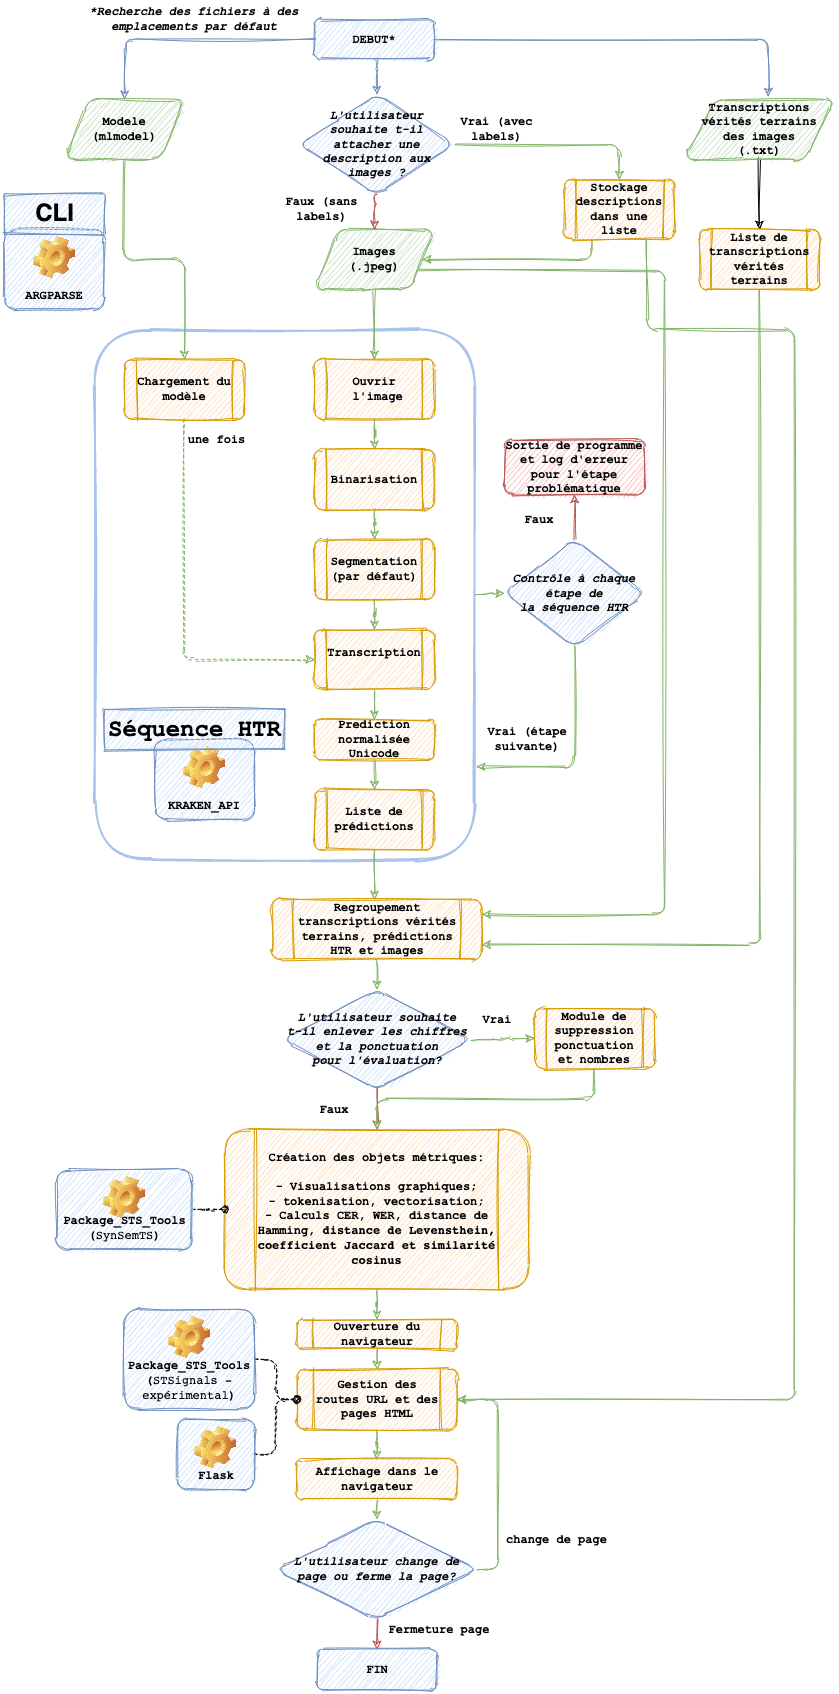
\includegraphics[width=18cm, height=22.5cm]{images_annexes/Kraken-Benchmark_modelisation.png}}}
    \caption{Algorigramme de \textit{Kraken-Benchmark}.   \textcopyright L. Terriel, 2020, Diagrams.net}
    \label{fig:algo-kb}
\end{figure}

\chapter{\textit{Scripts} Python complémentaires}
localisation : \citecode{/F-scripts\_python\_comp} contenant :

\begin{itemize}
    \item \citecode{script\_python\_POS.py} ou Figure \ref{fig:script_python_POS}
    \item \citecode{script\_python\_exif.py} ou Figure \ref{fig:script_python_exif}
    \item \citecode{script\_calc\_RO.py} ou Figure \ref{fig:script_calc_RO}
\end{itemize}

\begin{figure}[h]
\lstset{language=Python}
\begin{lstlisting}
"""
Exemple de script pour l'étiquetage morpho-syntaxique (part-of-speech)

Auteur : Lucas Terriel
Date : 14/09/2020
"""

# On importe le package spacy (tâches NLP)
import spacy
from spacy import displacy

# On charge un modèle français
# ! préalable télécharger le modèle (réseau convolutionnel entraîné sur deux corpus, WikiNER et Sequoia) !
# python -m spacy download fr_core_news_sm
model_fr = spacy.load("fr_core_news_sm")

# On défini une phrase de test
test = "Paul Charles Claude demeurant à Paris avec sa femme"

def return_POS(sentence):
    """
    fonction pour tokeniser la phrase et retourner les étiquettes grammaticale
    de chaque token.

    :param sentence: phrase
    :type sentence: str
    :return: token et étiquettes POS
    :type return : list
    """
    # Découpage de la phrase en mots (tokens)
    document = model_fr(sentence)
    # Retourne dans un dictionnaire les tokens (X) -clés- et leurs étiquettes (X.pos_) -valeurs- à partir d'une liste en compréhension
    return [{(X, X.pos_)} for X in document]

# affichage du dictionnaire
print(return_POS(test))

# Pour la visualisation dans le navigateur du POS on défini des paramètres de style
options = {"color": "red", "font": "Source Sans Pro"}

# Visualisation POS dans le navigateur
doc = model_fr(test)
displacy.serve(doc, style="dep", options=options)

\end{lstlisting}
\caption{\textit{Script} Python pour effectuer de l'étiquetage morpho-syntaxique (POS) \textcopyright L. Terriel, 2020}
\label{fig:script_python_POS}
\end{figure}

\begin{figure}[h]
\lstset{language=Python}
\begin{lstlisting}
"""
Exemple de script pour afficher les métadonnées EXIF d'une image

Auteur : Lucas Terriel
Date : 14/09/2020
"""

# import du module pyExifTool pour l'extraction de métadonnées Exif
import exiftool

# Création de l'objet ExifTool, on localise l'image et récupération des métadonnées dans un dictionnaire (possibilité de traiter en lot - batch)
with exiftool.ExifTool() as et:
    metadata = et.get_metadata('../static/Voyage_au_centre_de_la_
    [...]Verne_Jules_btv1b8600259v_16.jpeg')

# Affichage des métadonnées à partir du dictionnaire
for key, value in metadata.items():
    print(f'{key} => {value}')

\end{lstlisting}
\caption{\textit{Script} Python pour afficher les métadonnées Exif d'une image \textcopyright L. Terriel, 2020}
\label{fig:script_python_exif}
\end{figure}

\begin{figure}[h]
\lstset{language=Python}
\begin{lstlisting}
"""
Script pour afficher un score de similarité basé sur l'algorithme Ratcliff/Obershelp

Auteur : Lucas Terriel
Date : 14/09/2020
"""

# On importe le module built-in implémentant l'algorithme Ratcliff/Obershelp
import difflib

# On récupère le score 
similarite_ro = difflib.SequenceMatcher(None, "En l'an 1920 par la procuration", "En l'an 1920 par le procureur").ratio()

# On affiche le score
print(f'Le score de similarité est de : {similarite_ro}')

>>> Le score de similarité est de : 0.8333333333333334

\end{lstlisting}
\caption{\textit{Script} Python pour calculer un score de similarité suivant l'algorithme Ratcliff/Obershelp  \textcopyright L. Terriel, 2020}
\label{fig:script_calc_RO}
\end{figure}
